%=======================02-713 LaTeX template, following the 15-210 template==================
%
%
%
%
%    1. Update the information in section "A," put your name and the name of 
%       the class and the number of the problem set
%    2. Write your answers in section "B" below. Precede answers for all 
%       parts of a question with the command "\question{n}{desc}" where n is
%       the question number and "desc" is a short, one-line description of 
%       the problem. There is no need to restate the problem.
%    3. If a question has multiple parts, precede the answer to part x with the
%       command "\part{x}".
%

\documentclass[11pt]{article}
\usepackage[mathscr]{euscript}


\newcommand\question[2]{\vspace{.25in}\hrule\textbf{#1: #2}\vspace{.5em}\hrule\vspace{.10in}}
\renewcommand\part[1]{\vspace{.10in}\textbf{(#1)}}


% plots
\usepackage{graphicx}
\graphicspath{ {./images/} }


\usepackage{amsmath, amssymb, amsthm} %AMS packages
\usepackage{mathtools, graphicx, enumitem} %generally recommended
\usepackage{mathrsfs} %symbols I like
\usepackage{hyperref} %personal preference
\usepackage{microtype, } %recommended by stackexchange, never tried them myself
\usepackage{nag, todonotes} %workflow stuff, doesn't affect final document

% Layout
\usepackage{fancyhdr}
\usepackage[margin=1in]{geometry}
\lhead{\NAME}
\chead{\ClassNumber , Assignment \ANUM}
\rhead{Due: \duedate}
\setlength{\parindent}{0pt}
\setlength{\parskip}{5pt plus 1pt}
\setlength{\headheight}{13.6pt}
\pagestyle{fancyplain}


%-------------------------------------------<commands>--------------------------------------------------------
%%%%%%%%%%%%%%%%%%%%%%%%%%%%%%%%%%%%%%%%%											Letter Symbols
\newcommand{\R}{\mathbb{R}}
\newcommand{\N}{\mathbb{N}}
\newcommand{\Z}{\mathbb{Z}}
\newcommand{\Q}{\mathbb{Q}}
\newcommand{\C}{\mathbb{C}}
\newcommand{\F}{\mathcal{F}}
\renewcommand{\H}{\mathcal{H}} %overwrites long-umlaut diacritic
\newcommand{\eps}{\varepsilon}
\newcommand{\Exp}{\mathbb{E}}
\newcommand{\Info}{\mathcal{F}}
\renewcommand{\P}{\mathbb{P}}
%%%%%%%%%%%%%%%%%%%%%%%%%%%%%%%%%%%%%%%%%											Brackets
\newcommand{\paren}[1]{\left( #1 \right)}
\newcommand{\bracket}[1]{\left[ #1 \right]}
\newcommand{\chevron}[1]{\langle #1 \rangle}
\newcommand{\norm}[2][ ]{\left\lVert #2 \right\rVert_{#1}}
\newcommand{\abs}[1]{\left\lvert #1 \right\rvert}
\newcommand{\floor}[1]{\left\lfloor #1 \right\rfloor}
\newcommand{\ceil}[1]{\left\lceil #1 \right\rceil}
%%%%%%%%%%%%%%%%%%%%%%%%%%%%%%%%%%%%%%%%%											Operators
\DeclareMathOperator{\supp}{supp}
\DeclareMathOperator{\trace}{tr}
\DeclareMathOperator{\lspan}{span}
\DeclareMathOperator{\conv}{conv} % stands for conv, as in convex hull
\DeclareMathOperator{\Int}{int} % stands for int, as in interior of a set
\DeclareMathOperator{\cl}{cl}
\DeclareMathOperator{\sgn}{sgn}
\newcommand{\indep}{\perp \!\!\! \perp}
\newcommand{\NormCDF}[1]{\Phi \left[ #1 \right]}
%%%%%%%%%%%%%%%%%%%%%%%%%%%%%%%%%%%%%%%%%%											Aarows
\newcommand{\into}{\hookrightarrow}
\newcommand{\onto}{\twoheadrightarrow}
\newcommand{\weakly}{\rightharpoonup}
\newcommand{\isom}{\cong}
\newcommand{\restr}[1]{{\upharpoonright}_{#1}}
%\newcommand{\rest}{\big|}
%%%%%%%%%%%%%%%%%%%%%%%%%%%%%%%%%%%%%%%%%%											Common Abbreviations
\renewcommand{\th}{^\mathrm{th}} %overwrites thorn (old english letter)
\newcommand{\n}{^{-1}}
\newcommand{\half}{\frac{1}{2}}
%%%%%%%%%%%%%%%%%%%%%%%%%%%%%%%%%%%%%%%%%%											Differential Operators
\newcommand{\del}{\partial}
\newcommand{\grad}{\nabla}
\newcommand{\Laplace}{\Delta}
\renewcommand{\div}{\operatorname{div}} %overwrites division symbol
\newcommand{\dd}{\mathrm{d}}
\newcommand{\intd}{\,\dd}
\newcommand{\ddt}{\frac{\dd}{\dd t}}
\newcommand{\deriv}[2]{\frac{\dd #1}{\dd #2}} %can leave top blank, e.g. \deriv{}{x}
\newcommand{\pderiv}[2]{\frac{\partial #1}{\partial #2}} %ditto
%%%%%%%%%%%%%%%%%%%%%%%%%%%%%%%%%%%%%%%%%%											Favorite Functions and Space Names
\newcommand{\test}{\mathcal{D}}
\newcommand{\Ctest}{C_c^\infty}
\newcommand{\BMO}{\operatorname{BMO}}
\newcommand{\indic}[1]{\chi_{\{#1\}}}
\newcommand{\Leb}[2][\R^n]{L^{#2}(#1)}
%-------------------------------------------</commands>--------------------------------------------------------


\begin{document}\raggedright


%Section A==============Change the values below to match your information==================
\newcommand\NAME{Ki Hyun}  % your name
\newcommand\ClassNumber{FINM 36702}
\newcommand\ClassName{Portfolio Credit Risk: Modeling and Estimation}    
\newcommand\ANUM{4}              % the homework number
\newcommand\duedate{18:00 (CT) April 20 2023}	% due date
%Section B==============Put your answers to the questions below here=======================

\title{Assignment \ANUM}
\author{\NAME \\ 
\ClassNumber \text{:} \ClassName}
\date{Due: \duedate}

\maketitle

%\question{1}{Description of problem}
%\part{a}

\question{1}{EL, ELGD, EcLGD}

\begin{itemize}

\item EL:

$$
\begin{aligned}
\Exp[Loss] &= \sum_{states} \P\{state\} 
\times cPD_{state} \times cLGD_{state} \\
&= 0.40 \times 0.02 \times 0.10 \\
+& 0.30 \times 0.04 \times 0.30 \\
+& 0.20 \times 0.06 \times 0.50 \\
+& 0.10 \times 0.08 \times 0.70 \\
&= 0.016 
\end{aligned}
$$

\item ELGD:

$$
ELGD = \frac{EL}{PD}
$$

Here,

$$
\begin{aligned}
\P\{D\} &= \sum_{states} \P\{D \mid state \} 
\times \P\{state\} \\
&= 0.02 \times 0.40 +
0.04 \times 0.30 +
0.06 \times 0.20 +
0.08 \times 0.10 \\
&= 0.04 
\end{aligned}
$$

Therefore,

$$
ELGD = \frac{EL}{PD}
= \frac{0.016}{0.04}
= 0.4
$$

\item EcLGD:

$$
\begin{aligned}
\Exp[Loss \mid D] &= \sum_{states} \P\{state\} 
\times cLGD_{state} \\
&= 0.40 \times 0.10 
+ 0.30 \times 0.30 
+ 0.20 \times 0.50 
+ 0.10 \times 0.70 \\
&= 0.30
\end{aligned}
$$

\end{itemize}

\newpage

\question{2}{"Variant A" LGD function}

Given the LGD function:

$$
f_{cLGD}(cPD \mid a, PD, EL, ELGD, \rho) = 
ELGD^a \times
\frac{
\Phi \left[
\Phi^{-1}[cPD]
- \frac{\Phi^{-1}[PD]
- \Phi^{-1}[\frac{EL}{ELGD^a}]}
{\sqrt{1 - \rho}}
\right]
}
{cPD}
$$

Here, across various $a$, $PD$ was given as 0.05;
$ELGD$ was given as 0.3; $\rho$ was given as 0.15.

$EL$ may appear missing; however, it may be calculated 
using the relation between $PD$ and $ELGD$ as:

$$
EL = PD \times ELGD = 0.015
$$

Plotting the function above with $cPD$ on the x-axis
for $a \in \{-1, 0, 1, 2\}$ is shown as below:

\begin{figure}[h]
\centering
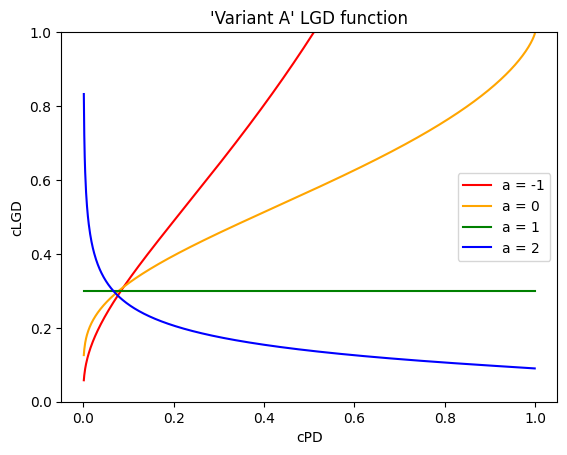
\includegraphics[scale=0.8]{Q2.png}
\caption{"Variant A" LGD functions}
\label{Fig:Q1}
\end{figure}


\newpage

\question{3}{Co-monotonic cPD and cLoss}

Co-monotonic $cPD$ and $cLoss$ that follows the same
distribution family means that the quantiles of the 
two values should match precisely.

Therefore, if we get the CDF values of $cPD$ from
the $Vasicek[PD = 0.02, \rho = 0.10]$ distribution
and plug the quantile back into the inverse-CDF function
prescribing $cLoss$ from the $Vasicek[El = 0.01, \rho]$
for each of the $\rho$ values, we would be able to get
$cLoss$ values from the $cPD$ values.

Then, we can create a LGD function plot using the relationship:

$$
cLGD = \frac{cLoss}{cPD}
$$

\begin{figure}[h]
\centering
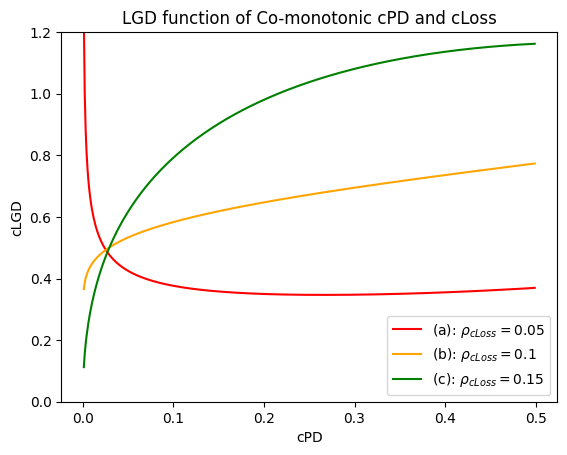
\includegraphics[scale=0.8]{Q3.png}
\caption{Co-monotonic Vasicek cPD and cLoss}
\label{Fig:Q1}
\end{figure}

\begin{itemize}

\item (a):

When $\rho = 0.05$, the $cLGD$ and $cPD$ does not resemble
co-monotonicity. Moreover, the $cLGD$ function gets rather 
flat as $cPD$ increases. It would be hard to find situations
where this LGD function is useful since, generally, $cLGD$ 
increases as default rate increases.

\item (b):

The $cLGD$ increases monotonically with $cPD$ values, as 
expected from real-life cases. This LGD-function seems to
be the most useful

\newpage

\item (c):

The $cLGD$ increases monotonically yet more rapidly than
in (b). Such rapid slope would be useful for extremely 
turbulent times. However, this LGD function has a critical 
flaw since the $cLGD$ values exceed $1.0$, which, in context, 
is nonsensical. Therefore, overall, the LGD function would 
not be useful.

\end{itemize}


\question{4}{ELGD, EL, PD}

The relevant assumptions of Question 3(b) is:

$$
\begin{aligned}
PD &= 0.02 \\
EL &= 0.01
\end{aligned}
$$

Now using the relationship between $ELGD$, $EL$, and $PD$,
the $ELGD$ value can be computed as:

$$
ELGD = \frac{EL}{PD} = \frac{0.01}{0.02} = 0.5
$$

\end{document}

$$
\begin{aligned}
\end{aligned}
$$